%
% This is a borrowed LaTeX template file for lecture notes for CS267,
% Applications of Parallel Computing, UCBerkeley EECS Department.
% Now being used for CMU's 10725 Fall 2012 Optimization course
% taught by Geoff Gordon and Ryan Tibshirani.  When preparing 
% LaTeX notes for this class, please use this template.
%
% To familiarize yourself with this template, the body contains
% some examples of its use.  Look them over.  Then you can
% run LaTeX on this file.  After you have LaTeXed this file then
% you can look over the result either by printing it out with
% dvips or using xdvi. "pdflatex template.tex" should also work.
%

\documentclass[twoside]{article}
\setlength{\oddsidemargin}{0.25 in}
\setlength{\evensidemargin}{-0.25 in}
\setlength{\topmargin}{-0.6 in}
\setlength{\textwidth}{6.5 in}
\setlength{\textheight}{8.5 in}
\setlength{\headsep}{0.75 in}
\setlength{\parindent}{0 in}
\setlength{\parskip}{0.1 in}

%
% ADD PACKAGES here:
%

\usepackage{amsmath,amsfonts,graphicx}

%
% The following commands set up the lecnum (lecture number)
% counter and make various numbering schemes work relative
% to the lecture number.
%
\newcounter{lecnum}
\renewcommand{\thepage}{\thelecnum-\arabic{page}}
\renewcommand{\thesection}{\thelecnum.\arabic{section}}
\renewcommand{\theequation}{\thelecnum.\arabic{equation}}
\renewcommand{\thefigure}{\thelecnum.\arabic{figure}}
\renewcommand{\thetable}{\thelecnum.\arabic{table}}

%
% The following macro is used to generate the header.
%
\newcommand{\lecture}[4]{
   \pagestyle{myheadings}
   \thispagestyle{plain}
   \newpage
   \setcounter{lecnum}{#1}
   \setcounter{page}{1}
   \noindent
   \begin{center}
   \framebox{
      \vbox{\vspace{2mm}
    \hbox to 6.28in { {\bf EE302 - Feedback Systems
	\hfill Spring 2019} }
       \vspace{4mm}
       \hbox to 6.28in { {\Large \hfill Lecture #1 \hfill} }
       \vspace{2mm}
       \hbox to 6.28in { {\it Lecturer: #2 \hfill } }
      \vspace{2mm}}
   }
   \end{center}
   \markboth{Lecture #1}{Lecture #1}

   \vspace*{4mm}
}
%
% Convention for citations is authors' initials followed by the year.
% For example, to cite a paper by Leighton and Maggs you would type
% \cite{LM89}, and to cite a paper by Strassen you would type \cite{S69}.
% (To avoid bibliography problems, for now we redefine the \cite command.)
% Also commands that create a suitable format for the reference list.
\renewcommand{\cite}[1]{[#1]}
\def\beginrefs{\begin{list}%
        {[\arabic{equation}]}{\usecounter{equation}
         \setlength{\leftmargin}{2.0truecm}\setlength{\labelsep}{0.4truecm}%
         \setlength{\labelwidth}{1.6truecm}}}
\def\endrefs{\end{list}}
\def\bibentry#1{\item[\hbox{[#1]}]}

%Use this command for a figure; it puts a figure in wherever you want it.
%usage: \fig{NUMBER}{SPACE-IN-INCHES}{CAPTION}
\newcommand{\fig}[3]{
			\vspace{#2}
			\begin{center}
			Figure \thelecnum.#1:~#3
			\end{center}
	}
% Use these for theorems, lemmas, proofs, etc.
\newtheorem{theorem}{Theorem}[lecnum]
\newtheorem{lemma}[theorem]{Lemma}
\newtheorem{proposition}[theorem]{Proposition}
\newtheorem{claim}[theorem]{Claim}
\newtheorem{corollary}[theorem]{Corollary}
\newtheorem{definition}[theorem]{Definition}
\newenvironment{proof}{{\bf Proof:}}{\hfill\rule{2mm}{2mm}}

% **** IF YOU WANT TO DEFINE ADDITIONAL MACROS FOR YOURSELF, PUT THEM HERE:

\begin{document}

% Lecture Details
\lecture{6}{Asst. Prof. M. Mert Ankarali}

\par 

\section{Transfer functions with multiple exogenous input}

When modeling and analyzing a closed system in addition to the desired reference input signal, it is also
important to model/analyze the system with unwanted disturbances and noise input signals. Let's 
consider the following block-diagram topology. In this closed-loop system, there exist three exogenous input
signals; $r(t)$ (reference input), $d(t)$ (``disturbance'' input), and $n(t)$ (``noise'' input).

  \begin{minipage}[h]{1\linewidth}
    \begin{center}
      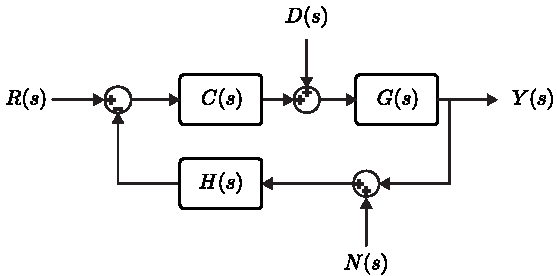
\includegraphics[width=0.8\textwidth]{dist}
    \end{center}
  \end{minipage}
  
  When modeling the response or characteristic of the system with respect to different external inputs, we assume that 
  remaining ones are zero.
  
  \paragraph{Response to $r(t)$}
  
  \begin{align*}
  	T_R(s) =  \frac{Y(s)}{R(s)} = \frac{C(s) G(s)}{1 + C(s) G(s) H(s)}
  \end{align*}
  
  \paragraph{Response to $d(t)$}
  
    \begin{align*}
  	T_D(s) =  \frac{Y(s)}{D(s)} =  \frac{G(s)}{1 + C(s) G(s) H(s)}
  \end{align*}
  
    \paragraph{Response to $n(t)$}
    
\begin{align*}
  	T_N(s) =  \frac{Y(s)}{N(s)} =  \frac{C(s) G(s) H(s)}{1 + C(s) G(s) H(s)}
  \end{align*}
 
  If we generalize, we can write $Y(s)$ as 
  
  \begin{align*}
  Y(s) = T_R(s) R(s) + T_D(s) D(s) + T_N(s) N(s)
  \end{align*}
  
  Lets roughly analyze the desired responses under different type of inputs. 
  Let's assume that $G(s)$ is the plant transfer function and $H(s)$ is the sensory 
  dynamics transfer function. $C(s)$ is the 
  transfer function of the controller.
  
  In the ideal case, we want 
  \begin{itemize}
  	\item Perfect tracking of reference signal, $T^*_R(s) \approx 1 $. 
	Since it is not possible to perfectly achieve this under dynamic system constrains,
	we can design a ``high gain'' controller such that 
	%
	  \begin{align*}
	  	T_R(s) \approx \frac{C(s) G(s)}{C(s) G(s) H(s)} \approx \frac{1}{H(s)}
	  \end{align*}
	  %
	  If $H(s) \approx 1$, then we can have a high tracking performance from the system. 
	  \item Perfect rejection of disturbance signal, $T^*_R(s) \approx 0 $. Similarly, 
	  we can design a ``high gain'' controller such that 
	  \begin{align*}
	  	T_D(s) \approx \frac{G(s)}{C(s) G(s) H(s)} \approx 0
	  \end{align*}
	  It seems that the requirement on $C(s)$ is similar for good tracking and
	  good disturbance rejection. 
	  \item Perfect rejection of noise signal, $T^*_N(s) \approx 0 $. In this case, we can design a 
	  ``low gain'' controller (or low gain $H(s)$) such that 
	  	  \begin{align*}
	  	T_N(s) \approx \frac{C(s) G(s) H(s)}{1} \approx 0
	  \end{align*}
  \end{itemize}
  
It seems that requirements on $C(s)$ and $H(s)$ start conflicting when we consider both tracking performance, disturbance rejection, and noise rejection. This paradox is the most well-known limitation of feedback control systems. The basic idea is that one can not only concentrate on designing a controller $C(s)$ such that we reach excellent closed-loop tracking performance when the system suffers from uncertainties and noises. Somehow we need to design $G(s)$, $H(s)$, and even $N(s)$ and $D(s)$ together such that the whole system achieves a ``good'' closed-loop behavior. 
  
  
% **** This ENDS THE EXAMPLES. DON'T DELETE THE FOLLOWING LINE:
\end{document}